\documentclass[conference]{IEEEtran}
\IEEEoverridecommandlockouts

\usepackage{cite}
\usepackage{amsmath,amssymb,amsfonts}
\usepackage{graphicx}
\usepackage{textcomp}
\usepackage{xcolor}
\usepackage{booktabs}
\usepackage{multirow}
\usepackage{colortbl}
\usepackage{float}
\usepackage{placeins}
\usepackage[caption=false,font=footnotesize]{subfig}
\usepackage[hidelinks]{hyperref}

\graphicspath{{./assets/}{./figures/}{./figures/generated/}{../assets/}{../figures/}{../figures/generated/}}

\definecolor{seafblue}{RGB}{238,245,252}
\definecolor{seafgreen}{RGB}{239,248,242}
\definecolor{seafwarm}{RGB}{253,242,240}

\setlength{\textfloatsep}{9pt plus 2pt minus 2pt}
\setlength{\floatsep}{8pt plus 2pt minus 2pt}
\setlength{\intextsep}{8pt plus 2pt minus 2pt}
\setlength{\dbltextfloatsep}{10pt plus 2pt minus 2pt}
\setlength{\dblfloatsep}{8pt plus 2pt minus 2pt}

\def\BibTeX{{\rm B\kern-.05em{\sc i\kern-.025em b}\kern-.08em
    T\kern-.1667em\lower.7ex\hbox{E}\kern-.125emX}}

\begin{document}
\raggedbottom

\title{DynaSEAF: Dynamics-Guided Transport for Ocean Anomaly Forecasting}

\author{
\IEEEauthorblockN{Shengxiang Yang\textsuperscript{1},
Zhibo Zhou\textsuperscript{1},
Xiaoyi Zhang\textsuperscript{1},
Yuchen Liu\textsuperscript{1}, and
Shiming Lin\textsuperscript{1,2,3}}
\IEEEauthorblockA{\textsuperscript{1}School of Informatics, Xiamen University, Xiamen, China}
\IEEEauthorblockA{\textsuperscript{2}School of Information Engineering, Changji University, Changji, China}
\IEEEauthorblockA{\textsuperscript{3}Key Laboratory of Southeast Coast Marine Information Intelligent Perception and Application, MNR, Zhangzhou, China\\
Corresponding author: xmulsm@xmu.edu.cn}
}

\maketitle

\begin{abstract}
Ocean temperature and salinity anomalies quantify departures from the expected seasonal state, yet their evolution is difficult to forecast across space, depth, and lead time. We introduce DynaSEAF, an incremental extension of the SEAF-v1 anomaly forecaster that couples direct anomaly prediction with model-generated dynamics. DynaSEAF predicts future UVEL, VVEL, SSHA, and MLD as training-only auxiliary targets, and uses the predicted dynamics to condition a learned effective deformation, a mask-aware transport branch, an adaptive direct/transport gate, and a lightweight residual correction. Anomaly persistence (AP) and damped anomaly persistence (DAP) remain external evaluation references. On validation, the 5.09-million-parameter DynaSEAF obtains TEMP RMSE $0.4940\pm0.0005$, SALT RMSE $0.0755\pm0.0002$, Macro $\mathrm{SS}_{\mathrm{AP}}=0.3637\pm0.0018$, and Macro $\mathrm{SS}_{\mathrm{DAP}}=0.2170\pm0.0022$. On the held-out 2011--2014 test split, it obtains TEMP RMSE $0.4750\pm0.0022$, SALT RMSE $0.0762\pm0.0004$, Macro $\mathrm{SS}_{\mathrm{AP}}=0.3522\pm0.0052$, and Macro $\mathrm{SS}_{\mathrm{DAP}}=0.2040\pm0.0066$, where all uncertainties are sample standard deviations over three seeds. The direct-anomaly target study remains a backbone-controlled result, reducing geometric MSE by $58.39\%$ for SEAF-v1 and $65.26\%$ for a Local CNN. A separate validation screen covers the A0--A4 ladder and four component controls at seed 42; we use it for descriptive component sensitivity and keep it separate from the three-seed test claim.
\end{abstract}

\renewcommand{\UrlFont}{\small\tt}
Code repository: \url{https://github.com/Mr-J-Forest/SEAF}\\
Data availability statement: Experiments use the ECMWF ORAS5/ICDC monthly reanalysis subset (1979--2014); the public product is available through the Copernicus Climate Data Store (DOI: 10.24381/cds.67e8eeb7)~\cite{copernicus2021oras5}. Preprocessing and evaluation details are provided in the accompanying repository.

\begin{IEEEkeywords}
Ocean prediction, anomaly forecasting, dynamics-guided transport, residual correction, persistence evaluation, temperature and salinity.
\end{IEEEkeywords}

\section{Introduction}

Temperature and salinity jointly characterize the ocean's thermohaline state and influence stratification, circulation, and air--sea exchange. Forecasting these depth-resolved fields from historical ocean states and external drivers is challenging because predictive information spans variables and spatial scales, while the target contains both a strong seasonal background and persistent transient structure.

Low physical-field error does not necessarily imply accurate prediction of anomaly evolution because the forecast also contains a comparatively regular climatological component. Let $Y_t$ denote the joint TEMP/SALT field and let $C_t$ denote the monthly climatology estimated from the training period only. The transient anomaly is
\begin{equation}
A_t=Y_t-C_t.
\label{eq:intro_anomaly}
\end{equation}
A standard full-field model is trained to map $X_{t-J+1:t}\mapsto Y_{t+h}$. Its error therefore reflects both reconstruction of the seasonal background and prediction of the transient anomaly. We instead train the model to predict the future anomaly directly:
\begin{equation}
\widehat{A}_{t+h}=f_{\theta}(X'_{t-J+1:t},h),\qquad
\widehat{Y}_{t+h}=C_{t+h}+\widehat{A}_{t+h}.
\label{eq:intro_direct}
\end{equation}
Here $X'$ contains the transformed history, causal tendency inputs, and external dynamics and forcing inputs. This anomaly-centered formulation directs the learning objective toward transient evolution while retaining physical-field reconstruction through $C_{t+h}$.

The separation from persistence is essential. An anomaly-persistence forecast is
\begin{equation}
\widehat{Y}^{\mathrm{AP}}_{t+h}=C_{t+h}+A_t,
\label{eq:intro_ap}
\end{equation}
and a damped anomaly-persistence forecast is
\begin{equation}
\widehat{Y}^{\mathrm{DAP}}_{t+h}=C_{t+h}+\rho_h A_t,
\label{eq:intro_dap}
\end{equation}
where $\rho_h$ is estimated from training histories. AP and DAP are external evaluation references: they are constructed by the evaluator rather than injected into the DynaSEAF forward path. Consequently, a zero anomaly output reconstructs the climatological background rather than AP.

We develop DynaSEAF as an incremental extension of the frozen SEAF-v1 anomaly forecaster. The inherited profile mixer processes the depth and history axes, local and low-mode spectral paths combine regional and nonlocal spatial information, and four decoder heads produce alternative deterministic anomaly hypotheses. DynaSEAF adds a future-dynamics auxiliary head, a learned effective deformation and differentiable anomaly warp, a direct/transport gate, and a lightweight residual correction. The future-dynamics labels are used only by the training auxiliary loss; the forecast path uses the model-generated dynamics and never receives future ground truth. The inherited LCFF path and raw external inputs remain part of the common backbone.

Direct anomaly prediction removes the burden of reconstructing the climatological background, but it still requires the model to represent displacement of persistent anomaly structures implicitly. DynaSEAF therefore augments the direct predictor with a dynamics-guided transport branch, while retaining a lightweight residual correction for evolution not explained by the transported field.

Our contributions are threefold:
\begin{enumerate}
    \item \textbf{Target formulation.} Under matched SEAF-v1 and Local-CNN controls, we show that direct anomaly forecasting substantially outperforms full-field prediction, establishing anomaly-centered prediction as the first-stage formulation.
    \item \textbf{DynaSEAF.} Building on this formulation, we augment direct anomaly prediction with a dynamics-guided transport branch and a lightweight residual correction, using model-predicted future dynamics without future-label leakage.
    \item \textbf{Persistence-aware empirical analysis.} We evaluate forecasts beyond climatology (CLIM), persistence (PERS), AP, and DAP across lead, depth, variable, and region, and compare the frozen DynaSEAF with SEAF-v1 and larger learned baselines. We report descriptive three-seed validation and test aggregates without a statistical-superiority claim over learned baselines.
\end{enumerate}

The A0--A4 ladder and component controls are evaluated on validation with the same 3,344 forecast origin--window samples and five-month horizon. The accompanying per-sample archive records the transport and correction diagnostics and supports descriptive mechanism plots; these validation-only diagnostics are not used for test checkpoint selection or test claims.

\section{Related Work}

\subsection{Persistence and Anomaly Prediction}
Persistence and climatology are strong references in slowly varying geophysical systems. Predictability studies compare forecasts with persistence-like references and damp anomalies using estimated temporal correlations~\cite{jacox2019dampedpersistence}. Earlier spatiotemporal ocean models also report gains relative to persistence, particularly at short leads~\cite{xiaoSpatiotemporalDeepLearning2019}. We predict future anomalies directly and use AP and DAP as external evaluation references, thereby testing whether a forecast contains information beyond the latest observed anomaly.

\subsection{Spectral and Spatiotemporal Forecasting}
Fourier-domain operators provide large spatial receptive fields through a small number of learned modes. FourCastNet introduced an adaptive Fourier neural operator for global weather forecasting~\cite{pathak2022fourcastnet}, while related systems use cascaded or three-dimensional neural designs for medium-range prediction~\cite{chen2023fuxi,bi2023accurate}. Recurrent models provide a complementary approach: ConvLSTM preserves local spatial structure while modeling recurrence~\cite{shiConvolutionalLSTMNetwork2015}, and PredRNN extends this design with spatiotemporal memory~\cite{wangPredRNNRecurrentNeural2017}. Recent sea-surface-temperature work combines ConvLSTM with deformable attention~\cite{shiSeaSurfaceTemperature2024}. DynaSEAF inherits SEAF-v1's low spatial Fourier modes as a compact nonlocal mixer and augments them with dynamics-guided transport refinement and residual correction.

\subsection{Data-Driven Ocean Models and Physical Inputs}
Data-driven ocean models complement numerical solvers by learning nonlinear dependencies from observations and prescribed drivers~\cite{boninoMachineLearningMethods2024,zhaoDeepLearningOcean2024}. Recent systems address eddy-resolving forecasting~\cite{cuiWenHaiForecastingEddying2025}, end-to-end global forecasting~\cite{elAouniGLONETMercatorEndtoEnd2024}, and three-dimensional or sub-daily prediction~\cite{huangFuXiOceanGlobalOcean2025,wuAxiomOceanForecastingThreeDimensional2026}. Multi-member forecasting is widely used to represent forecast uncertainty~\cite{molteni1996ecmwf}, including in recent data-driven ocean ensembles~\cite{huangFuXiONSDataDrivenEnsemble2026}. DynaSEAF instead uses parallel decoder heads to produce alternative deterministic anomaly hypotheses and combines them with a dynamics-guided transport refinement plus a lightweight residual correction; these hypotheses are not calibrated ensemble members or independent physical simulations.

Temporal differences and external drivers can provide information absent from a single static state. Multi-factor SST forecasts incorporate variables such as currents~\cite{yangMultiFactorDeepLearning2025}, while neural ocean-model corrections use state-dependent forcing and air--sea heat exchange~\cite{stortoCorrectionSeaSurface2025}. Long-lead ENSO prediction likewise illustrates that data-driven models can extract precursors from coupled ocean--atmosphere fields~\cite{hamDeepLearningMultiyear2019}. We evaluate temporal tendencies and external dynamics and forcing as distinct input groups under a fixed anomaly target.

\subsection{Dynamics-Guided and Transport-Based Spatiotemporal Forecasting}
Differentiable spatial transformation is the basic computational primitive behind several learned warping methods. Spatial Transformer Networks predict input-dependent transformation parameters and use a differentiable sampler to transform feature maps~\cite{jaderberg2015spatial}. DynaSEAF does not claim differentiable warping as a new operation: it uses the same general primitive for a forecasting-specific purpose. Its deformation is not introduced to learn transformation invariance in a feature representation; it transports the latest climatology-removed anomaly field, $A_t$, to a future anomaly hypothesis, $\widehat{A}^{\mathrm{trans}}_{t+h}=\mathcal{W}(A_t,\Delta_{t+h})$, with a depth-resolved deformation predicted for the ocean forecasting task.

Video forecasting has also used learned motion fields to preserve spatial structure. TrajGRU learns location-variant recurrent connections and warps previous hidden states along learned trajectories~\cite{shi2017trajgru}, whereas Deep Voxel Flow predicts a per-pixel spatiotemporal flow and synthesizes frames by interpolating values from an existing video volume~\cite{liu2017voxel}. These works motivate transporting existing structure instead of regenerating every future field from scratch. DynaSEAF differs in the object and source of the motion representation: its future-dynamics head predicts $\widehat{\mathrm{UVEL}}$, $\widehat{\mathrm{VVEL}}$, $\widehat{\mathrm{SSHA}}$, and $\widehat{\mathrm{MLD}}$ under training-only auxiliary supervision, and these model-generated physical-dynamics forecasts condition a learned effective deformation in the 3-D TEMP/SALT anomaly field. The predicted velocities are therefore not directly equated with a prescribed displacement.

Structured dynamics and residual modeling provide a second relevant precedent. PhyDNet separates a PDE-constrained latent physical branch from complementary unknown information~\cite{leguen2020phydnet}. More closely, NowcastNet combines a learned motion-driven evolution operator with intensity residuals for precipitation nowcasting~\cite{zhang2023nowcastnet}. We therefore do not present a transport-plus-residual decomposition as an unprecedented idea. DynaSEAF's distinction is its ocean-specific conditioning and forecast formulation: predicted future physical variables condition a depth-resolved deformation, the deformation warps the latest anomaly rather than a full physical field, and a direct anomaly branch remains available through an adaptive gate. The residual term $R_h$ is a lightweight correction for evolution not explained by the transported field, rather than a separately supervised forecast target. The resulting path is $\widehat{D}_{t+h}\!\rightarrow\!\Delta_{t+h}\!\rightarrow\!\mathcal{W}(A_t,\Delta_{t+h})$, combined with the direct branch as formalized later in Eq.~\eqref{eq:dynaseaf_forecast}.

\section{Data and Problem Definition}

\subsection{ORAS5 Dataset and Grid}
We use monthly ORAS5 ocean reanalysis from the ECMWF OCEAN5 system~\cite{zuo2019ocean5}, distributed through the Copernicus Climate Data Store~\cite{copernicus2021oras5}. The dataset spans January 1979--December 2014 and contains 432 monthly time steps on a $1^\circ$ grid with 180 latitudes, 360 longitudes, and 20 selected depth levels:
\[
\begin{gathered}
\{0,5,10,20,30,50,75\},\\
\{100,125,150,200,250,300,400\},\\
\{500,600,700,800,900,1000\}\ \mathrm{m}.
\end{gathered}
\]
The targets are TEMP and SALT at every selected level. Inputs additionally include zonal and meridional velocity (UVEL and VVEL), sea-surface-height anomaly (SSHA), mixed-layer depth (MLD), zonal and meridional wind stress (TAUX and TAUY), net heat flux (QNET), and freshwater flux (WFLUX). Depth profiles are retained in a structured tensor until profile mixing, after which one forward pass jointly predicts both target variables.

The sampler extracts $22\times33$ spatial windows with an $8^\circ$ stride and retains 76 ocean-only windows per forecast origin. An ocean mask derived from TEMP at 1000~m defines valid spatial windows, while variable-specific masks restrict evaluation to finite target values.
% Reproducibility record retained from the pre-revision draft: finite fractions were 0.6473 for surface-forcing inputs and 0.5957 for depth-resolved TEMP/SALT fields; no configured variable or complete time slice was missing.

\subsection{Forecast Task and Splits}
Each sample maps a 12-month history to the next five monthly states. The chronological split spans January 1979--December 2006 for training, January 2007--December 2010 for validation, and January 2011--December 2014 for testing. After constructing valid history--forecast pairs, these segments contain 320, 44, and 44 forecast origins, respectively; each of the validation and test sets contains 3,344 origin--window samples. For the first validation or test forecast origin, the input history may include preceding months from the earlier chronological segment; all forecast targets remain strictly within the designated validation or test period.

For every variable, monthly climatology and normalization statistics are estimated from the training period only and then applied unchanged to validation and test data. Causal tendency inputs use one-step backward differences, and variable-specific validity masks are retained throughout preprocessing. The learning target is the normalized future anomaly; physical-space evaluation reverses the normalization and adds the corresponding training-period climatology.

\subsection{Reference Forecasts and Skill}
The evaluator constructs four deterministic references with the same target layout:
\begin{align}
\widehat{Y}^{\mathrm{CLIM}}_{t+h}&=C_{t+h},\\
\widehat{Y}^{\mathrm{PERS}}_{t+h}&=Y_t,\\
\widehat{Y}^{\mathrm{AP}}_{t+h}&=C_{t+h}+(Y_t-C_t),\\
\widehat{Y}^{\mathrm{DAP}}_{t+h}&=C_{t+h}+\rho_h(Y_t-C_t).
\label{eq:references}
\end{align}
The damping coefficients are estimated from training histories for each target variable, lead, and depth channel. Model skill relative to AP is
\begin{equation}
\mathrm{SS}_{\mathrm{AP}}=1-\frac{\mathrm{MSE}_{\mathrm{model}}}{\mathrm{MSE}_{\mathrm{AP}}},
\label{eq:ssap}
\end{equation}
and $\mathrm{SS}_{\mathrm{DAP}}$ is defined analogously. A positive score indicates lower MSE than the corresponding external evaluation reference over the same valid target points; aggregate skill need not be positive at every lead or depth.

\section{DynaSEAF: Dynamics-Guided Anomaly Forecasting}

\subsection{Architecture Overview}
Figure~\ref{fig:architecture} summarizes the complete DynaSEAF pipeline. A schema-aware encoder with hidden width 192 first processes anomaly profiles, causal tendencies, and the available external history. The inherited SEAF-v1 backbone combines profile mixing, two local--global spatial blocks, four deterministic direct-anomaly hypotheses, and lead-conditioned forcing fusion. Its direct forecast is retained as one branch, while a future-dynamics head predicts training-supervised UVEL, VVEL, SSHA, and MLD signals from the shared representation. Those model-generated dynamics condition an effective deformation, a mask-aware transport warp, a target-resolved gate, and a lightweight residual correction. The future climatology is restored only after anomaly fusion; AP and DAP are constructed separately during evaluation.

\begin{figure*}[!t]
\centering

\includegraphics[width=\textwidth]{dynaseaf_architecture}
\caption{DynaSEAF architecture. The inherited SEAF-v1 backbone produces a direct anomaly branch and a shared representation for the dynamics-guided extension. A future-dynamics head predicts UVEL, VVEL, SSHA, and MLD only for the training auxiliary loss; its model-generated output conditions deformation, mask-aware transport, adaptive gating, and a lightweight residual correction. The fused anomaly is combined with future climatology to obtain the physical TEMP/SALT forecast. AP/DAP are external evaluation references, not model inputs.}
\label{fig:architecture}
\end{figure*}

\subsection{Direct Anomaly Target}
Let $X^+$ denote the history after input augmentation and let $A_{t+h}$ denote the future anomaly in physical space. The direct branch of DynaSEAF reuses the SEAF-v1 forecast:
\begin{equation}
\widehat{A}_{t+h}=f_{\theta}(X^+,h),\qquad
\widehat{Y}_{t+h}=C_{t+h}+\widehat{A}_{t+h}.
\label{eq:seaf_target}
\end{equation}
DynaSEAF retains this direct forecast as one branch and does not treat AP or DAP as model inputs. Its transport branch uses the latest anomaly as a source field, while the gate, deformation, and residual correction are learned from the history and model-generated dynamics. AP and DAP are constructed only by the evaluator. The target comparison is therefore between direct anomaly prediction and a matched direct full-field objective, rather than between alternative implementations of an AP residual.

\subsection{Profile and Local--Global Encoders}
DynaSEAF first reuses the structured SEAF-v1 encoder, which restores the shape of each input window,
\begin{equation}
X\in\mathbb{R}^{B\times J\times V\times Z\times H\times W},
\label{eq:profile_shape}
\end{equation}
where $V$ is the number of target variables, $Z$ is the number of depth levels, and the remaining inputs are handled through the augmented channel set. A depth mixer applies a grouped 1-D convolution along $Z$ independently for each variable--month pair, and a temporal mixer applies a grouped 1-D convolution along $J$ independently for each variable--depth pair. A pointwise projection then combines the structured profile features into hidden channels. This ordering preserves the physical meaning of the depth and history axes until after profile mixing.

Each local--global block combines a residual $3\times3$ convolutional path with the low-mode Fourier path described below. The local path retains compact spatial structure, while the spectral path supplies a nonlocal receptive field; learned scaling combines the two updates. DynaSEAF adds its dynamics-guided heads after this inherited feature representation.

\subsection{Input Information Groups}
The tendency group contains causal one-step backward differences,
\begin{equation}
\Delta V_t=V_t-V_{t-1},
\label{eq:tendency}
\end{equation}
for the TEMP/SALT profiles. The external group contains UVEL, VVEL, SSHA, MLD, TAUX, TAUY, QNET, and WFLUX. These variables are inputs rather than future targets and use the same training-period preprocessing as the base fields. DynaSEAF uses UVEL, VVEL, SSHA, and MLD as the future-dynamics auxiliary targets during training, while the forward path consumes only the dynamics predicted from the history. The complete external group remains available to the shared backbone.

\subsection{Low-Mode Spatial Spectral Mixer}
The input features are encoded through three parallel branches: the schema-aware profile encoder $\mathbf{F}_{\mathrm{prof}}$, the tendency context encoder $\mathbf{F}_{\mathrm{tend}}$, and the scaled external forcing encoder $\alpha_{\mathrm{forc}}\mathbf{F}_{\mathrm{forc}}$ with learnable scale $\alpha_{\mathrm{forc}}$. Their additive combination,
\begin{equation}
\mathbf{F}_0 = \mathbf{F}_{\mathrm{prof}} + \mathbf{F}_{\mathrm{tend}} + \alpha_{\mathrm{forc}}\mathbf{F}_{\mathrm{forc}},
\end{equation}
is sent to two cascaded Local--Global spatial blocks. Each block combines a local residual $3\times3$ Conv2D path with a global spectral path. In the spectral path, the feature map $U$ is transformed via
\begin{equation}
\widehat{U}=\mathrm{rFFT2}(U),
\end{equation}
retains an $8\times8$ low-frequency rectangle, applies learned complex diagonal weights to the frequency bands, and reconstructs spatial features via inverse FFT:
\begin{equation}
U'=U+\psi\left(\mathrm{iFFT2}\left(\mathcal{M}_{\mathrm{low}}(\widehat{U})\right)\right).
\label{eq:spectral}
\end{equation}
The resulting representation $F\in\mathbb{R}^{B\times192\times H\times W}$ is shared across subsequent prediction heads.

\subsection{Multiple Deterministic Hypotheses}
The shared feature map is sent to $M=4$ parallel decoder heads. Each head contains a Conv2D--GroupNorm--GELU block followed by a $1\times1$ projection to the $K C_y$ joint target channels. The resulting deterministic hypotheses are
\begin{equation}
\widehat{A}_m=\mathcal{D}_{m,\theta}(F),\qquad m=1,\ldots,M.
\end{equation}
The decoder heads represent alternative deterministic anomaly hypotheses rather than independent physical simulations or calibrated uncertainty estimates.

\subsection{Lead-Conditioned Forcing Fusion}
LCFF couples the dedicated scaled forcing encoder with lead-conditioned hypothesis routing. Given the $M=4$ deterministic hypothesis fields, a lead-specific learnable logit vector $\mathbf{w}_h \in \mathbb{R}^M$ produces global lead-conditioned aggregation weights:
\begin{equation}
G_m(h)=\operatorname{softmax}_m(\mathbf{w}_h)_m.
\label{eq:lcff}
\end{equation}
The direct anomaly forecast for lead $h \in \{1,\ldots,K\}$ is
\begin{equation}
\widehat{A}^{\mathrm{dir}}_h=\sum_{m=1}^{M}G_m(h)\widehat{A}_{m,h}.
\label{eq:lcff_aggregate}
\end{equation}
The SEAF-v1 LCFF control disables both the dedicated forcing representation and lead-conditioned aggregation, while retaining the raw external inputs, profile mixer, local--global blocks, spectral settings, four deterministic hypotheses, and uniform head averaging. This historical backbone contrast does not isolate either LCFF component and is not interpreted as a DynaSEAF component ablation.

\subsection{Dynamics-Guided Transport Refinement}
Given the shared SEAF-v1 feature map $F$ and a lead embedding $e_h$, DynaSEAF predicts a compact set of future dynamics,
\begin{equation}
\begin{aligned}
\widehat{D}_h&=H_{\mathrm{dyn}}(F,e_h),\\[-1pt]
D&\in\{\mathrm{UVEL},\mathrm{VVEL},\mathrm{SSHA},\mathrm{MLD}\}.
\end{aligned}
\label{eq:dynaseaf_dynamics}
\end{equation}
For the frozen ORAS5 schema, the prediction horizon is $K=5$ and the future-dynamics channel count is $C_{\mathrm{dyn}}=42$. The channels are packed as
\begin{equation}
\widehat{D}_h=\big[\widehat{D}_{h,\mathrm{UVEL}},\widehat{D}_{h,\mathrm{VVEL}},
\widehat{D}_{h,\mathrm{SSHA}},\widehat{D}_{h,\mathrm{MLD}}\big],
\end{equation}
where $\widehat{D}_{h,\mathrm{UVEL}},\widehat{D}_{h,\mathrm{VVEL}}\in\mathbb{R}^{20\times H\times W}$ cover all 20 depth levels used by TEMP/SALT, while $\widehat{D}_{h,\mathrm{SSHA}},\widehat{D}_{h,\mathrm{MLD}}\in\mathbb{R}^{1\times H\times W}$ are surface scalar maps. Thus one lead has shape $[B,42,H,W]$ and the stacked head output has shape $[B,K,42,H,W]$, with channel slices $[0,20)$, $[20,40)$, $[40,41)$, and $[41,42)$, respectively. Each field is first converted to a training-period monthly climatology anomaly and then standardized with one variable-specific training-only standard scaler; for UVEL/VVEL, that scaler pools the 20 depth channels and spatial cells, and the fitted scalers are reused for validation and test. The future labels are used only in the training auxiliary loss. Although SSHA and MLD remain single surface channels rather than being copied to every depth, the deformation, gate, and residual-correction heads concatenate all 42 predicted dynamics channels with $F$ and $e_h$ before their $1\times1$ projections, allowing the learned surface signals to condition all depth-level outputs.

The model then predicts a learned effective deformation in grid-cell units,
\begin{equation}
\begin{aligned}
\Delta_h&=H_{\mathrm{def}}(F,\widehat{D}_h,e_h),\\[-1pt]
\Delta_h&\in[-d_{\max},d_{\max}]^{B\times20\times H\times W\times2},
\qquad d_{\max}=1.0.
\end{aligned}
\label{eq:dynaseaf_deformation}
\end{equation}
where the last axis stores the two horizontal components $(\Delta x,\Delta y)$ and the bound is one grid cell. In the frozen TEMP/SALT schema, one 2-D deformation field is predicted for each of the 20 depth levels. TEMP and SALT share the deformation field at a given depth through the target-to-deformation map $[0,\ldots,19,0,\ldots,19]$; the model therefore predicts 20 fields rather than 40 independent displacement fields. A mask-aware differentiable warp $W$ transports the latest anomaly source field:
\begin{equation}
\widehat{A}^{\mathrm{trans}}_h
 =W(A_t,\Delta_h).
\label{eq:dynaseaf_transport}
\end{equation}
The warp samples values and validity masks separately and renormalizes valid ocean values, so land and non-finite source values do not dilute a valid target cell.

The final anomaly forecast combines the direct prediction, transported prediction, and residual innovation:
\begin{align}
R_h&=H_{\mathrm{innov}}(F,\widehat{D}_h,e_h),\nonumber\\
g_h&=\sigma\!\left(H_{\mathrm{gate}}(F,\widehat{D}_h,e_h)\right),\nonumber\\
\widehat{A}_h&=(1-g_h)\odot\widehat{A}^{\mathrm{dir}}_h
       +g_h\odot\widehat{A}^{\mathrm{trans}}_h+R_h.
\label{eq:dynaseaf_forecast}
\end{align}
The residual innovation $R_h$ is a learned non-transport anomaly correction for local physical tendencies and thermodynamic modifications not captured by coordinate advection. The gate output layer pre-activation bias is initialized to $b_0 \approx -1.7346$, setting the initial post-sigmoid gate prior to $\sigma(b_0) \approx 0.15$. The residual-correction and gate layers are zero-initialized, keeping the initial model close to the direct SEAF-v1 forecast while allowing lead- and location-dependent corrections. The physical prediction is then reconstructed as $\widehat{Y}_{t+h}=C_{t+h}+\mathcal{T}^{-1}(\widehat{A}_h)$, where $\mathcal{T}^{-1}$ denotes inverse target standardization.

For DynaSEAF, the training objective is
\begin{equation}
\begin{aligned}
\mathcal{L}_{\mathrm{dyn}}
&=\frac{1}{4}
  \sum_{q\in\{\mathrm{UVEL},\mathrm{VVEL},\mathrm{SSHA},\mathrm{MLD}\}}
  \operatorname{MSE}_{\mathrm{valid}}(\widehat{D}_q,D_q),\\
\mathcal{L}
&=\frac{1}{2}\mathcal{L}_{\mathrm{TEMP}}
  +\frac{1}{2}\mathcal{L}_{\mathrm{SALT}}\\
  &\quad+\lambda_{\mathrm{dyn}}\mathcal{L}_{\mathrm{dyn}}.
\end{aligned}
\label{eq:dynaseaf_loss}
\end{equation}
with $\lambda_{\mathrm{dyn}}=0.10$. Here $\operatorname{MSE}_{\mathrm{valid}}$ selects the declared channel slice for one variable and averages squared errors over its valid batch, lead, channel, and spatial elements; the four resulting variable-level losses are then averaged uniformly by $1/4$. Consequently, the 20-channel UVEL/VVEL fields do not receive twenty times the weight of the one-channel SSHA/MLD maps, and invalid future-label elements are excluded rather than pooled as zeros. Future dynamics labels are absent from validation and test inputs, and checkpoint selection remains based only on the weighted TEMP/SALT validation objective.

\subsection{Objective}
The inherited direct branch is optimized with a variable-weighted mean-squared-error objective in transformed anomaly space:
\begin{equation}
\mathcal{L}_{\mathrm{MSE}}=\sum_{v\in\{\mathrm{TEMP},\mathrm{SALT}\}}\lambda_v\,
\mathrm{MSE}(\widehat{A}_v,A_v),\qquad \sum_v\lambda_v=1.
\label{eq:loss}
\end{equation}
The full DynaSEAF objective is given in Eq.~\eqref{eq:dynaseaf_loss}; checkpoints are selected by validation weighted MSE on TEMP/SALT only.

\begin{figure*}[!t]
\centering
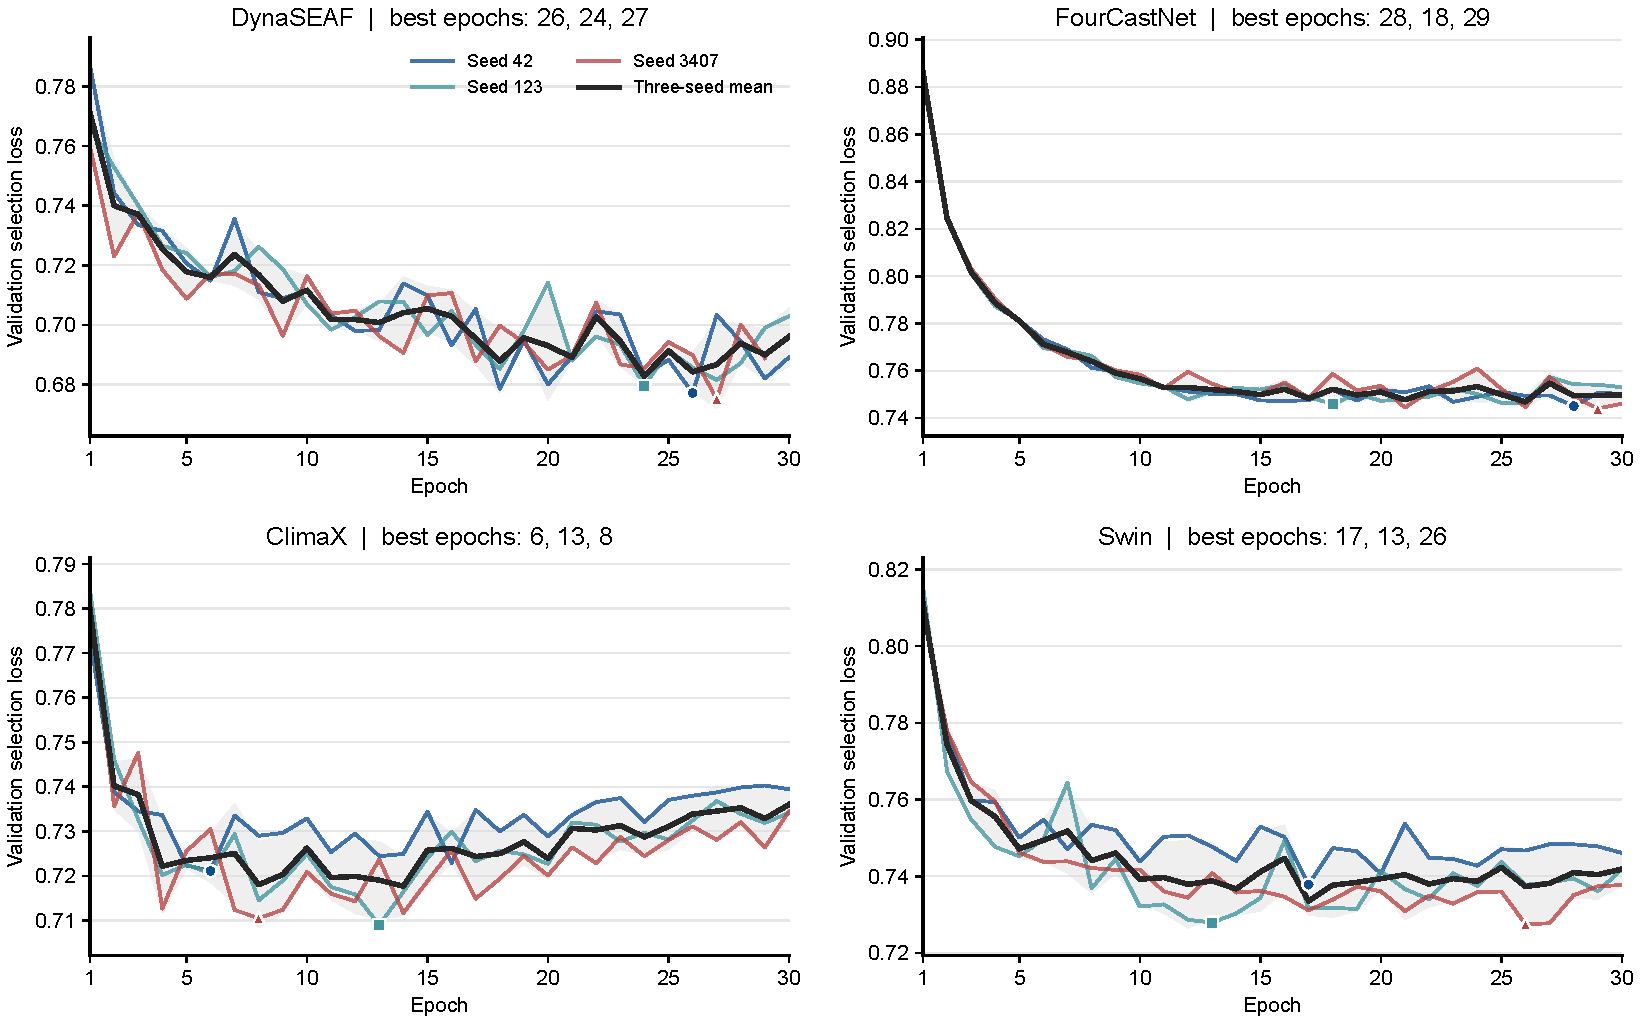
\includegraphics[width=0.96\textwidth]{fig_validation_convergence}
\caption{Validation convergence assessment for the proposed DynaSEAF and the three learned comparison models under the common 30-epoch budget. Colored lines show seeds 42, 123, and 3407; the black line is their mean, and the gray band denotes one sample standard deviation. Markers identify the validation-best checkpoint for each seed. SEAF-v1 is reserved for the internal backbone comparison in Tables~\ref{tab:incremental} and~\ref{tab:validation_main}. The recovered seed-3407 DynaSEAF event log contains validation values through epoch 29; its unavailable epoch-30 value is left blank rather than imputed.}
\label{fig:validation_convergence}
\end{figure*}

\section{Experimental Protocol}

\subsection{Campaign and Reproducibility}
We train every learned configuration for 30 epochs with random seeds 42, 123, and 3407. Unless stated otherwise, tables report the mean $\pm$ sample standard deviation across these seeds. The target-formulation and baseline studies use the same chronological splits, preprocessing, window sampler, evaluation masks, optimization budget, and checkpoint-selection rule. For every run, we retain the checkpoint with the lowest validation weighted MSE rather than the final-epoch checkpoint. After architecture screening, the frozen DynaSEAF configuration---the hidden-width-192 SEAF-v1 backbone plus future-dynamics auxiliary prediction, learned effective deformation, transport branch, target-resolved gate, and residual correction---is confirmed on validation. The A0--A4 ladder and the four component controls are a validation-only screen at seed 42, with no test iteration or retraining during diagnostic export. The test split is evaluated only after the main DynaSEAF configuration and its checkpoints are frozen.

Figure~\ref{fig:validation_convergence} assesses whether the common 30-epoch budget disadvantages the proposed DynaSEAF model or its learned comparators. All four plotted models enter a stable validation regime within the allotted budget, although their validation-best checkpoints occur at different epochs. DynaSEAF reaches its seed-wise minima at epochs 26, 24, and 27. ClimaX reaches its minima earliest and subsequently overfits, whereas Swin stabilizes after its initial descent. FourCastNet has late per-seed minima at epochs 28 and 29, but its three-seed mean is already nearly flat after approximately 12--15 epochs, and its epoch-30 losses are only $0.27$--$0.95\%$ above the corresponding minima. The inherited SEAF-v1 convergence trace is not repeated in this main-model assessment because its role is the internal backbone comparator reported in Tables~\ref{tab:incremental} and~\ref{tab:validation_main}. The seed-3407 DynaSEAF event artifact records no epoch-30 validation scalar, so the figure leaves that point blank and does not infer it from the final checkpoint evaluation. We therefore interpret 30 epochs as a common optimization budget under validation-best checkpointing, without claiming that every optimizer trajectory has reached an identical or fully converged endpoint.

\subsection{Learned Baselines}
The deterministic references are CLIM, PERS, AP, and DAP from Eq.~\eqref{eq:references}. For the main learned-anomaly comparison, all learned models use the same historical input information and TEMP/SALT direct-anomaly forecasting target; DynaSEAF additionally uses future UVEL, VVEL, SSHA, and MLD as training-only auxiliary supervision, which is unavailable at validation and test inference. The explicitly labelled full-field controls are confined to the separate target-formulation experiment. SEAF-v1 is the inherited direct-anomaly comparator; the local CNN control retains the complete input set but replaces the spectral--ensemble backbone. FourCastNet, ClimaX, and Swin adapters use the OceanForecastBench implementations at commit \texttt{3a53d97}~\cite{han2026oceanforecastbench,oceanforecastbenchCode2025}. All learned baselines are retrained from scratch under the same data and preprocessing protocol. Because their parameter counts are not matched to DynaSEAF, the comparison measures predictive performance rather than parameter-controlled architectural effects.

\subsection{Controlled Target and LCFF Contrasts}
The target-formulation study compares direct anomaly prediction with a matched full-field objective while holding the backbone, inputs, optimizer, training schedule, loss weighting, and checkpoint protocol fixed. We conduct this backbone-controlled comparison on SEAF-v1 and on a distinct Local CNN control; a tuned SEAF-v1 full-field control changes only the learning rate from $3\times10^{-4}$ to $8\times10^{-4}$. The Local CNN conditions use three seeds, 30 epochs, and the same 44 origins per seed. DynaSEAF is evaluated as the frozen mainline extension. Its A0--A4 ladder and component controls are evaluated on validation as a seed-42 diagnostic screen; their per-sample values are reported separately from the three-seed mainline aggregates. AP and DAP remain external evaluation references throughout.

\subsection{Metrics and Paired Contrasts}
We report physical-space RMSE for TEMP and SALT, Macro $\mathrm{SS}_{\mathrm{AP}}$, and Macro $\mathrm{SS}_{\mathrm{DAP}}$. Macro scores give TEMP and SALT equal weight after their variable-specific MSE skills are computed. Lead-wise and depth-wise scores use the same valid-point masks as the aggregate evaluator.

Because the $22\times33$ windows use an $8^\circ$ stride, a physical grid point can occur in more than one window. We do not deduplicate these occurrences. Aggregate metrics therefore weight each finite target point by the number of origin--window samples in which it appears, and the same sampler and weighting rule are applied to every model and split. The terminal-anchor rule prevents uncovered edges when the domain extent is not divisible by the stride.

Forecast origins define the paired units. We draw 10,000 moving-block bootstrap replicates with block length five and seed 20260826. Benjamini--Hochberg (BH) correction is applied across comparisons. The primary statistic is the log MSE ratio, $\log(\mathrm{MSE}_{\mathrm{reference}}/\mathrm{MSE}_{\mathrm{candidate}})$, for which positive values favor the candidate. The corresponding geometric MSE reduction is $1-\exp(-\overline{\log(\mathrm{MSE}_{\mathrm{reference}}/\mathrm{MSE}_{\mathrm{candidate}})})$. We report paired block-bootstrap $p$ values and BH-adjusted $q$ values. Paired reductions and seed-averaged Macro $\mathrm{SS}_{\mathrm{AP}}$ summarize related but distinct comparisons.

\FloatBarrier
\section{Results}
\label{sec:results}

\subsection{Target Formulation: Why Anomaly Forecasting?}
The first stage of the progression asks what the model should predict. The paired analysis in Table~\ref{tab:target_contrast} is a backbone-controlled result rather than a DynaSEAF component ablation. Direct anomaly prediction reduces equal-variable geometric MSE by $58.39\%$ relative to the matched SEAF-v1 full-field control (95\% CI: $56.71$--$59.91\%$; $p=0.0002$; $q=0.00055$), and by $58.45\%$ relative to the tuned control.

The same contrast holds for the distinct 0.995-million-parameter Local CNN: its anomaly/full-field conditions attain Macro $\mathrm{SS}_{\mathrm{AP}}=0.2516\pm0.0039$/$-1.3570\pm0.0781$ and TEMP/SALT RMSE $0.5249\pm0.0005$/$0.0802\pm0.0004$ versus $0.9418\pm0.0174$/$0.1276\pm0.0011$. Its paired origin-level reduction is $65.26\%$ (95\% CI: $64.04$--$66.50\%$). Thus, the target effect persists across two compact backbones under the shared protocol and motivates the anomaly target inherited by DynaSEAF.

\begin{table}[!t]
\centering
\caption{Paired validation target contrasts between direct anomaly prediction and full-field controls. Positive reduction indicates lower geometric MSE for direct anomaly prediction; $q$ is BH-adjusted. The Local CNN comparison uses a distinct compact backbone under the same validation protocol.}
\label{tab:target_contrast}
\footnotesize
\setlength{\tabcolsep}{4pt}
\renewcommand{\arraystretch}{1.12}
\begin{tabular}{lccc}
\toprule
Backbone / reference objective & Reduction $\uparrow$ & 95\% CI & $q$\\
\midrule
SEAF-v1 / matched full-field & $\mathbf{58.39\%}$ & $[56.71,59.91]$ & 0.00055\\
SEAF-v1 / tuned full-field & $\mathbf{58.45\%}$ & $[56.04,61.18]$ & 0.00055\\
Local CNN / matched full-field & $\mathbf{65.26\%}$ & $[64.04,66.50]$ & 0.00020\\
\bottomrule
\end{tabular}
\end{table}

The validation aggregate is consistent with the paired contrasts: all SEAF-v1 full-field controls and the Local CNN full-field control have negative skill relative to AP and DAP. The result supports the first arrow, full-field prediction $\rightarrow$ anomaly prediction, independently of the later DynaSEAF component comparison.

\subsection{DynaSEAF Incremental Confirmation: Why Structured Anomaly Evolution?}
The controlled incremental comparison in Table~\ref{tab:incremental} isolates the frozen DynaSEAF extension from its SEAF-v1 direct-anomaly backbone. The extension adds 116,866 parameters for the lead embedding, future-dynamics head, deformation head, residual-correction head, and adaptive gate. On validation, DynaSEAF reduces the mean TEMP and SALT RMSE and increases both persistence-relative skill scores. These are aggregate confirmation results; component sensitivity is examined separately in the validation ablation screen and is not folded into this three-seed comparison.

\begin{table}[!t]
\centering
\caption{Three-seed validation comparison between the inherited SEAF-v1 backbone and the frozen DynaSEAF extension (mean $\pm$ sample standard deviation).}
\label{tab:incremental}
\scriptsize
\setlength{\tabcolsep}{3.0pt}
\renewcommand{\arraystretch}{1.04}
\textit{(a) Physical-space error and model size}\\[2pt]
\begin{tabular}{lccc}
\toprule
Setting & Params (M) & TEMP RMSE $\downarrow$ & SALT RMSE $\downarrow$\\
\midrule
\rowcolor{seafblue} SEAF-v1 & 4.97 & $0.5061\!\pm\!0.0042$ & $0.0769\!\pm\!0.0003$\\
DynaSEAF & 5.09 & $\mathbf{0.4940\!\pm\!0.0005}$ & $\mathbf{0.0755\!\pm\!0.0002}$\\
\bottomrule
\end{tabular}\\[4pt]
\textit{(b) Persistence-relative skill}\\[2pt]
\begin{tabular}{lcc}
\toprule
Setting & Macro SS$_{\rm AP}$ $\uparrow$ & Macro SS$_{\rm DAP}$ $\uparrow$\\
\midrule
\rowcolor{seafblue} SEAF-v1 & $0.3176\!\pm\!0.0023$ & $0.1646\!\pm\!0.0033$\\
DynaSEAF & $\mathbf{0.3637\!\pm\!0.0018}$ & $\mathbf{0.2170\!\pm\!0.0022}$\\
\bottomrule
\end{tabular}
\end{table}

To quantify the frozen extension against its inherited backbone, we reused the existing origin-level validation reports for all three seeds and applied the same forecast-origin moving-block bootstrap specified above. Table~\ref{tab:dynaseaf_paired} reports the geometric MSE reduction $1-\exp\!\left(-\overline{\log\!\left(\mathrm{MSE}_{\mathrm{SEAF-v1}}/\mathrm{MSE}_{\mathrm{DynaSEAF}}\right)}\right)$ together with its 95\% bootstrap interval, two-sided bootstrap $p$, and BH-adjusted $q$. The macro equal-variable reduction is $4.23\%$ (95\% CI $3.11$--$5.31\%$); this is frozen validation evidence against SEAF-v1, not a test-set selection or a statistical-superiority claim over the other learned baselines.

\begin{table}[!t]
\centering
\caption{Paired validation comparison of frozen DynaSEAF with the inherited SEAF-v1 backbone. The statistic is the geometric MSE reduction from the forecast-origin moving-block bootstrap (10,000 replicates, block length five); $p$ is two-sided and $q$ is BH-adjusted.}
\label{tab:dynaseaf_paired}
\scriptsize
\setlength{\tabcolsep}{3.5pt}
\renewcommand{\arraystretch}{1.05}
\begin{tabular}{lcccc}
\toprule
Metric & Reduction $\uparrow$ & 95\% CI & $p$ & $q$ \\
\midrule
TEMP & $4.54\%$ & $[2.40,6.45]$ & 0.00020 & 0.00020 \\
SALT & $3.92\%$ & $[2.74,4.97]$ & 0.00020 & 0.00020 \\
Macro (equal variable weight) & $4.23\%$ & $[3.11,5.31]$ & 0.00020 & 0.00020 \\
\bottomrule
\end{tabular}
\end{table}

\subsection{Validation Comparison with Learned Baselines}
With the target and incremental gain established, Table~\ref{tab:validation_main} places the frozen DynaSEAF configuration alongside SEAF-v1 and anomaly-target adapters trained under the same validation protocol. DynaSEAF attains Macro $\mathrm{SS}_{\mathrm{AP}}=0.3637\pm0.0018$ and Macro $\mathrm{SS}_{\mathrm{DAP}}=0.2170\pm0.0022$, the highest means among the listed models. It also has the lowest reported TEMP and SALT RMSE means. DynaSEAF uses 5.09 million parameters: 4.97 million are inherited from the direct SEAF-v1 forecaster and 0.12 million belong to the dynamics-guided extension. These results establish a numerical validation advantage under the frozen protocol, but do not establish statistical superiority over the learned baselines.

\begin{table}[!t]
\centering
\caption{Validation performance over three random seeds (mean $\pm$ sample standard deviation). DynaSEAF is the main model; SEAF-v1 is its inherited direct-anomaly comparator. All rows use the same data protocol and direct anomaly target.}
\label{tab:validation_main}
\scriptsize
\setlength{\tabcolsep}{3.0pt}
\renewcommand{\arraystretch}{1.05}
\textit{(a) Physical-space error and model size}\\[2pt]
\begin{tabular}{lccc}
\toprule
Method & Params (M) & TEMP RMSE $\downarrow$ & SALT RMSE $\downarrow$\\
\midrule
\rowcolor{seafblue} SEAF-v1 & 4.97 & $0.5061\!\pm\!0.0042$ & $0.0769\!\pm\!0.0003$\\
DynaSEAF & 5.09 & $\mathbf{0.4940\!\pm\!0.0005}$ & $\mathbf{0.0755\!\pm\!0.0002}$\\
FourCastNet & 20.05 & $0.5174\!\pm\!0.0009$ & $0.0793\!\pm\!0.0001$\\
ClimaX & 61.62 & $0.5108\!\pm\!0.0017$ & $\mathbf{0.0767\!\pm\!0.0005}$\\
Swin & 35.72 & $0.5169\!\pm\!0.0027$ & $0.0777\!\pm\!0.0003$\\
\bottomrule
\end{tabular}\\[4pt]
\textit{(b) Persistence-relative skill}\\[2pt]
\begin{tabular}{lcc}
\toprule
Method & Macro SS$_{\rm AP}$ $\uparrow$ & Macro SS$_{\rm DAP}$ $\uparrow$\\
\midrule
\rowcolor{seafblue} SEAF-v1 & $0.3176\!\pm\!0.0023$ & $0.1646\!\pm\!0.0033$\\
DynaSEAF & $\mathbf{0.3637\!\pm\!0.0018}$ & $\mathbf{0.2170\!\pm\!0.0022}$\\
FourCastNet & $0.2899\!\pm\!0.0023$ & $0.1287\!\pm\!0.0025$\\
ClimaX & $\mathbf{0.3253\!\pm\!0.0086}$ & $\mathbf{0.1705\!\pm\!0.0099}$\\
Swin & $0.3075\!\pm\!0.0049$ & $0.1490\!\pm\!0.0061$\\
\bottomrule
\end{tabular}
\end{table}

\subsection{Held-out Test Evaluation}
Table~\ref{tab:test_main} reports the frozen DynaSEAF checkpoints evaluated once on the 2011--2014 test period. The test manifest records no test access before checkpoint freezing, no training or checkpoint reselection, and serial evaluation of \texttt{best\_model.pth} only. DynaSEAF obtains normalized RMSE $0.8090\pm0.0037$, physical TEMP/SALT RMSE $0.4750\pm0.0022$/$0.0762\pm0.0004$, and Macro $\mathrm{SS}_{\mathrm{AP}}/\mathrm{SS}_{\mathrm{DAP}}=0.3522\pm0.0052/0.2040\pm0.0066$. It has the best mean physical error and persistence-relative skill among the listed models, while the table should be read as a descriptive three-seed comparison rather than a statistical-superiority test. The test period was not used for checkpoint selection, width selection, or component interpretation.

\begin{table}[!t]
\centering
\caption{Held-out 2011--2014 test performance over three random seeds (mean $\pm$ sample standard deviation).}
\label{tab:test_main}
\scriptsize
\setlength{\tabcolsep}{3.0pt}
\renewcommand{\arraystretch}{1.05}
\textit{(a) Physical-space error and model size}\\[2pt]
\begin{tabular}{lccc}
\toprule
Method & Params (M) & TEMP RMSE $\downarrow$ & SALT RMSE $\downarrow$\\
\midrule
\rowcolor{seafblue} SEAF-v1 & 4.97 & $0.4913\!\pm\!0.0037$ & $0.07919\!\pm\!0.00047$\\
DynaSEAF & 5.09 & $\mathbf{0.4750\!\pm\!0.0022}$ & $\mathbf{0.07616\!\pm\!0.00038}$\\
FourCastNet & 20.05 & $0.4928\!\pm\!0.0020$ & $0.07993\!\pm\!0.00008$\\
ClimaX & 61.62 & $\mathbf{0.4891\!\pm\!0.0025}$ & $\mathbf{0.07837\!\pm\!0.00036}$\\
Swin & 35.72 & $0.4961\!\pm\!0.0011$ & $0.07858\!\pm\!0.00005$\\
\bottomrule
\end{tabular}\\[4pt]
\textit{(b) Persistence-relative skill}\\[2pt]
\begin{tabular}{lcc}
\toprule
Method & Macro SS$_{\rm AP}$ $\uparrow$ & Macro SS$_{\rm DAP}$ $\uparrow$\\
\midrule
\rowcolor{seafblue} SEAF-v1 & $0.2822\!\pm\!0.0076$ & $0.1238\!\pm\!0.0098$\\
DynaSEAF & $\mathbf{0.3522\!\pm\!0.0052}$ & $\mathbf{0.2040\!\pm\!0.0066}$\\
FourCastNet & $0.2822\!\pm\!0.0048$ & $0.1217\!\pm\!0.0056$\\
ClimaX & $\mathbf{0.3053\!\pm\!0.0037}$ & $\mathbf{0.1485\!\pm\!0.0040}$\\
Swin & $0.2941\!\pm\!0.0011$ & $0.1340\!\pm\!0.0007$\\
\bottomrule
\end{tabular}
\end{table}

\begin{table*}[!t]
\centering
\caption{Global lead-wise performance of the frozen DynaSEAF checkpoints on the held-out 2011--2014 test split. Values are mean $\pm$ sample standard deviation over seeds 42, 123, and 3407. SS$_{\rm AP}$ and SS$_{\rm DAP}$ are computed against the corresponding AP/DAP MSE at the same variable and lead; physical RMSE is reported in $^\circ$C for TEMP and PSU for SALT.}
\label{tab:test_leadwise}
\scriptsize
\setlength{\tabcolsep}{3.2pt}
\renewcommand{\arraystretch}{1.05}
\begin{tabular}{c|cc|cc|cc}
\toprule
Lead & TEMP SS$_{\rm AP}$ $\uparrow$ & SALT SS$_{\rm AP}$ $\uparrow$ & TEMP SS$_{\rm DAP}$ $\uparrow$ & SALT SS$_{\rm DAP}$ $\uparrow$ & TEMP RMSE $\downarrow$ & SALT RMSE $\downarrow$ \\
\midrule
1 & $0.267\!\pm\!0.003$ & $0.297\!\pm\!0.003$ & $0.184\!\pm\!0.003$ & $0.247\!\pm\!0.003$ & $0.3504\!\pm\!0.0006$ & $0.0542\!\pm\!0.0001$ \\
2 & $0.339\!\pm\!0.005$ & $0.344\!\pm\!0.006$ & $0.178\!\pm\!0.006$ & $0.253\!\pm\!0.007$ & $0.4569\!\pm\!0.0018$ & $0.0714\!\pm\!0.0003$ \\
3 & $0.380\!\pm\!0.007$ & $0.360\!\pm\!0.008$ & $0.171\!\pm\!0.009$ & $0.245\!\pm\!0.010$ & $0.4960\!\pm\!0.0027$ & $0.0792\!\pm\!0.0005$ \\
4 & $0.399\!\pm\!0.006$ & $0.364\!\pm\!0.007$ & $0.160\!\pm\!0.009$ & $0.233\!\pm\!0.009$ & $0.5172\!\pm\!0.0027$ & $0.0840\!\pm\!0.0005$ \\
5 & $0.406\!\pm\!0.009$ & $0.366\!\pm\!0.006$ & $0.145\!\pm\!0.012$ & $0.224\!\pm\!0.007$ & $0.5322\!\pm\!0.0039$ & $0.0874\!\pm\!0.0004$ \\
\bottomrule
\end{tabular}
\end{table*}

The global lead-wise test metrics in Table~\ref{tab:test_leadwise} are computed from the same frozen per-seed evaluation reports as Table~\ref{tab:test_main}; no checkpoint, architecture, or hyperparameter was selected from these test values. AP skill increases from lead 1 to lead 5 for both variables, whereas DAP skill decreases gradually; physical RMSE increases with lead for both TEMP and SALT.

\begin{figure*}[!t]
\centering
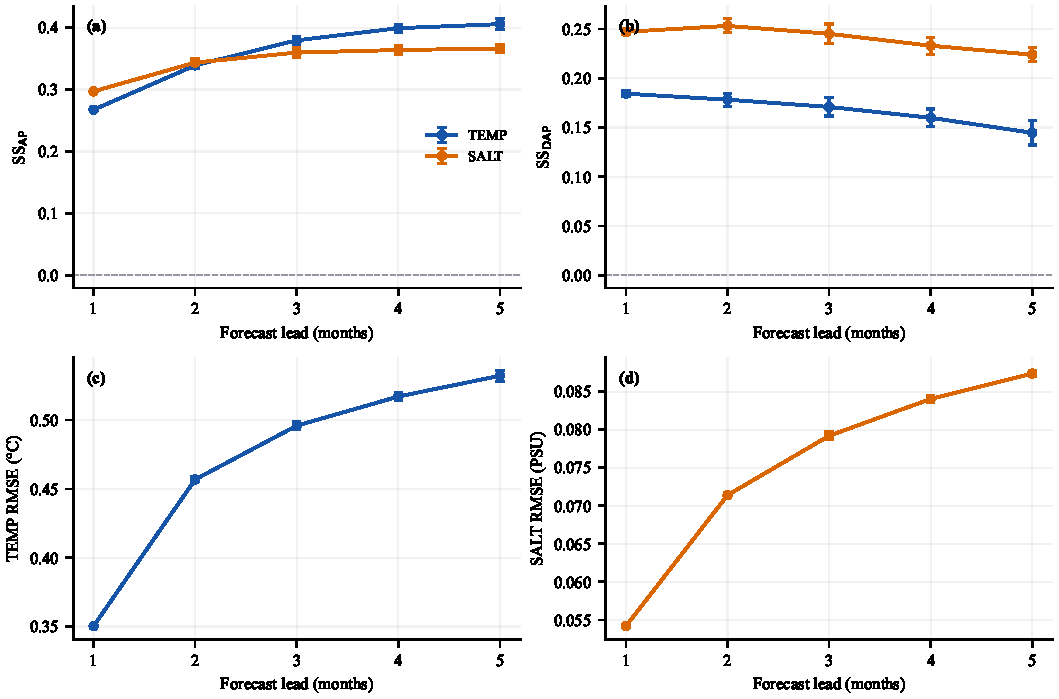
\includegraphics[width=0.98\textwidth]{main_test_leadwise_metrics}
\caption{Global lead-wise held-out test metrics for frozen DynaSEAF. The top row reports variable-specific skill relative to AP and DAP; the bottom row reports physical RMSE. Curves show the mean over seeds 42, 123, and 3407 and error bars show sample standard deviation. These plots are descriptive summaries of fixed-checkpoint evaluation.}
\label{fig:test_leadwise}
\end{figure*}

\subsection{Depth-Resolved Test Skill}
Depth stratification of the frozen DynaSEAF test results shows positive AP skill across the sampled depths. At 0~m, TEMP/SALT AP skill is $0.326\pm0.017$/$0.369\pm0.007$; at 200~m it is $0.378\pm0.009$/$0.350\pm0.005$; and at 1000~m it is $0.268\pm0.006$/$0.262\pm0.003$. The model therefore retains information beyond anomaly persistence in the deepest sampled layer, although the magnitude is smaller than at 200~m for both variables. These values are descriptive three-seed means; the complete depth-resolved metrics remain in the archived test reports.

\subsection{DynaSEAF Validation Ablations}
We next use the validation split to inspect a focused incremental ladder and the transport control. This screen is intentionally reported at seed 42 and in the diagnostic metric space: each value is the mean normalized RMSE over the $3{,}344$ validation origin--window samples, five leads, and valid grid points for the indicated variable. It is therefore not a replacement for the three-seed global validation/test aggregates in Tables~\ref{tab:validation_main} and~\ref{tab:test_main}. The focused table does not assume that the full DynaSEAF row dominates every configuration; it isolates the transport sensitivity without turning one seed into an inferential claim. The complete component screen is reported in Appendix~\ref{sec:appendix_validation_ablation}.

\begin{table}[!t]
\centering
\caption{Focused validation ablation screen for DynaSEAF (seed 42). Entries are means over validation origin--window samples and leads of normalized RMSE; lower is better. The complete component screen is provided in Appendix~\ref{sec:appendix_validation_ablation}.}
\label{tab:dynaseaf_ablations}
\scriptsize
\setlength{\tabcolsep}{3.0pt}
\renewcommand{\arraystretch}{1.05}
\begin{tabular}{lccc}
\toprule
Configuration & TEMP $\downarrow$ & SALT $\downarrow$ & Macro $\downarrow$\\
\midrule
A0: SEAF-v1 & 0.8127 & 0.7354 & 0.7741\\
A1: dynamics only & 0.8147 & 0.7396 & 0.7771\\
A2: + transport & 0.7961 & 0.7203 & 0.7582\\
A4: full DynaSEAF & 0.7980 & 0.7201 & 0.7591\\
\texttt{no\_transport} & 0.8198 & 0.7400 & 0.7799\\
\bottomrule
\end{tabular}
\end{table}

The focused screen shows that adding the transport branch produces the clearest reduction relative to A0: Macro normalized RMSE decreases from $0.7741$ to $0.7582$. The no-transport control is the weakest displayed DynaSEAF variant at $0.7799$, whereas A4 retains the transport gain at $0.7591$. Transport is therefore the clearest sensitivity in the DynaSEAF design. The complete component screen is retained in Appendix~\ref{sec:appendix_validation_ablation}; all values are validation-screen patterns from one seed rather than test-level claims.

\subsection{Per-Sample Mechanism Evidence}
For every validation configuration, the diagnostic archive contains $33{,}440$ rows: $3{,}344$ origin--window samples, five forecast leads, and two target variables. The accompanying manifest records the direct forecast, transported forecast, residual correction (stored as the model's innovation tensor), adaptive gate, effective deformation, and predicted future-dynamics outputs, together with the split and checkpoint provenance. Future dynamics labels are not read by the forward path during this export, and the diagnostics do not participate in checkpoint selection.

\subsection{Mechanism Statistics and Qualitative Forecasts}
For the full DynaSEAF row, the mean gate decreases with lead from $0.797$ to $0.390$ for TEMP and from $0.825$ to $0.444$ for SALT. The corresponding mean absolute predicted-dynamics output decreases from $0.218$ to $0.075$ in normalized auxiliary space. The first two panels of Fig.~\ref{fig:dynaseaf_mechanism_validation} compare the final fused forecast with the direct and transport branches; they do not treat the residual correction as a standalone forecast. The counterfactual panel reports the paired per-sample difference between the full final RMSE and the matched forecast without the residual correction. Its sign changes with variable and lead, so the residual is interpreted as a conditional correction rather than as an independently supervised prediction target.

\begin{figure*}[!t]
\centering
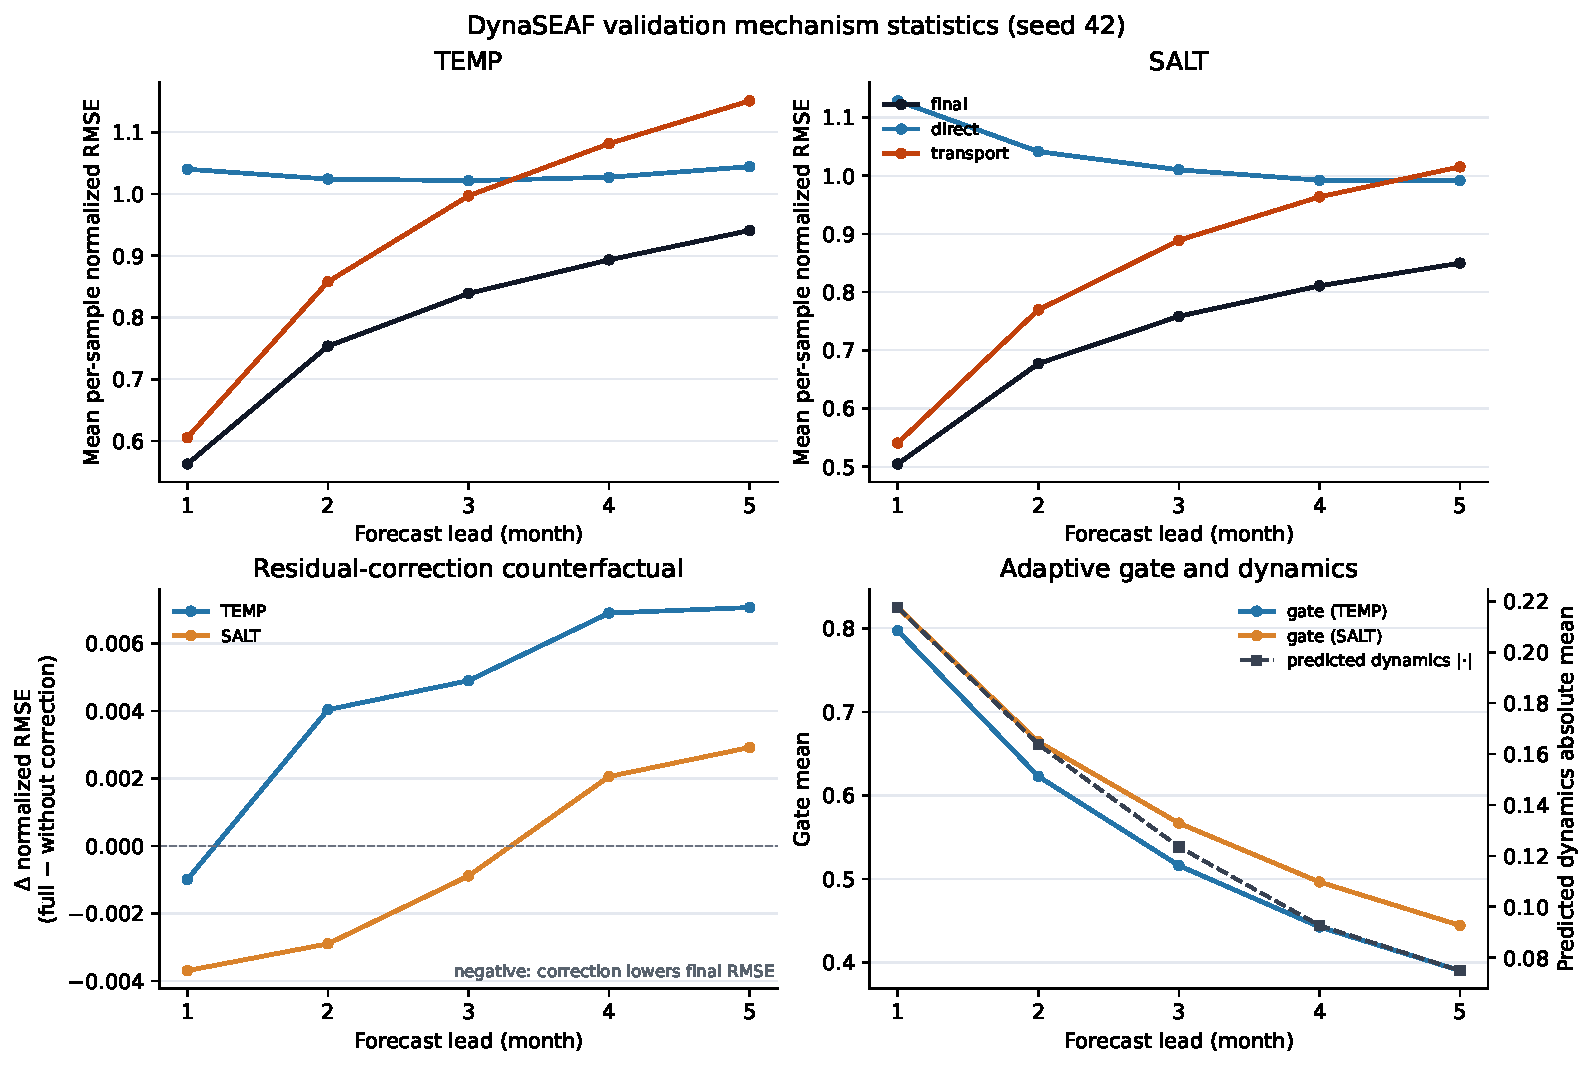
\includegraphics[width=\textwidth]{dynaseaf_mechanism_validation}
\caption{Validation-only mechanism statistics for full DynaSEAF at seed 42. The TEMP and SALT panels show normalized RMSE averaged over origin--window samples at each lead for the final, direct, and transport branches. The residual-correction panel shows the paired per-sample $\Delta$RMSE between the full final forecast and the matched forecast without the residual correction; negative values favor retaining the correction. The last panel shows target-resolved gate means and the mean absolute predicted-dynamics output.}
\label{fig:dynaseaf_mechanism_validation}
\end{figure*}

\begin{figure*}[!t]
\centering
\subfloat[TEMP validation branches]{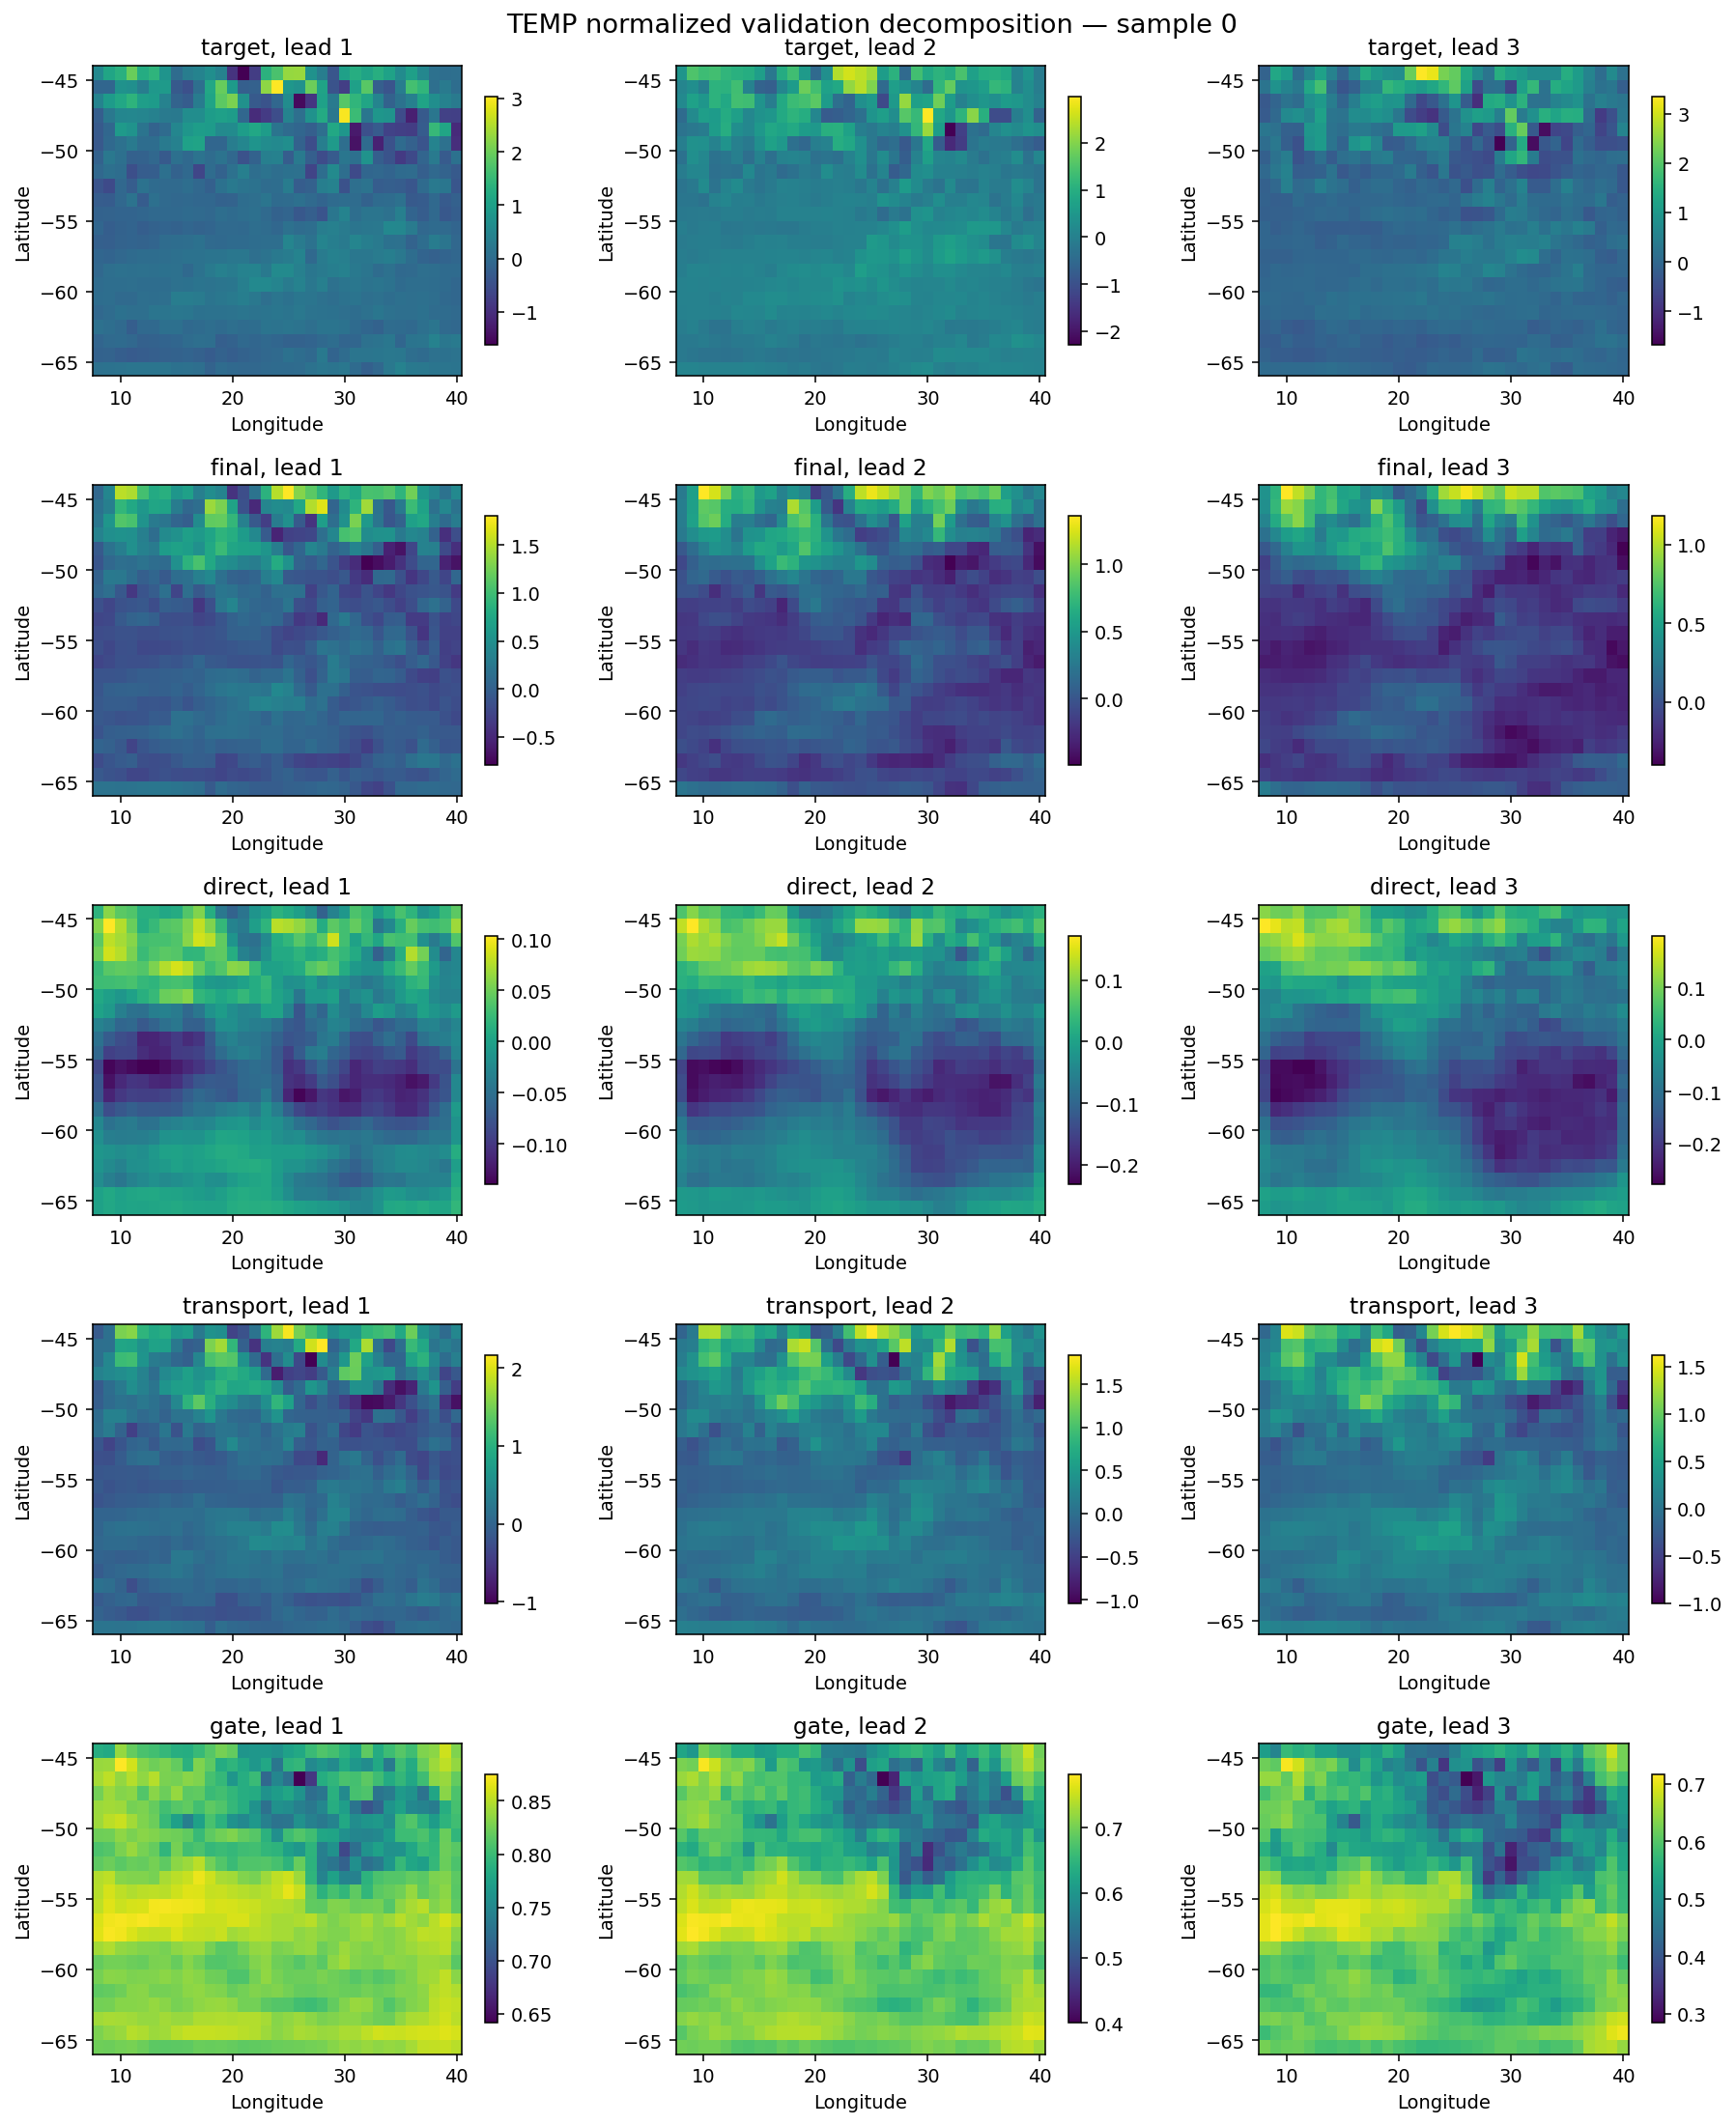
\includegraphics[width=0.46\textwidth]{dynaseaf_validation_temp_panel}}\hfill
\subfloat[SALT validation branches]{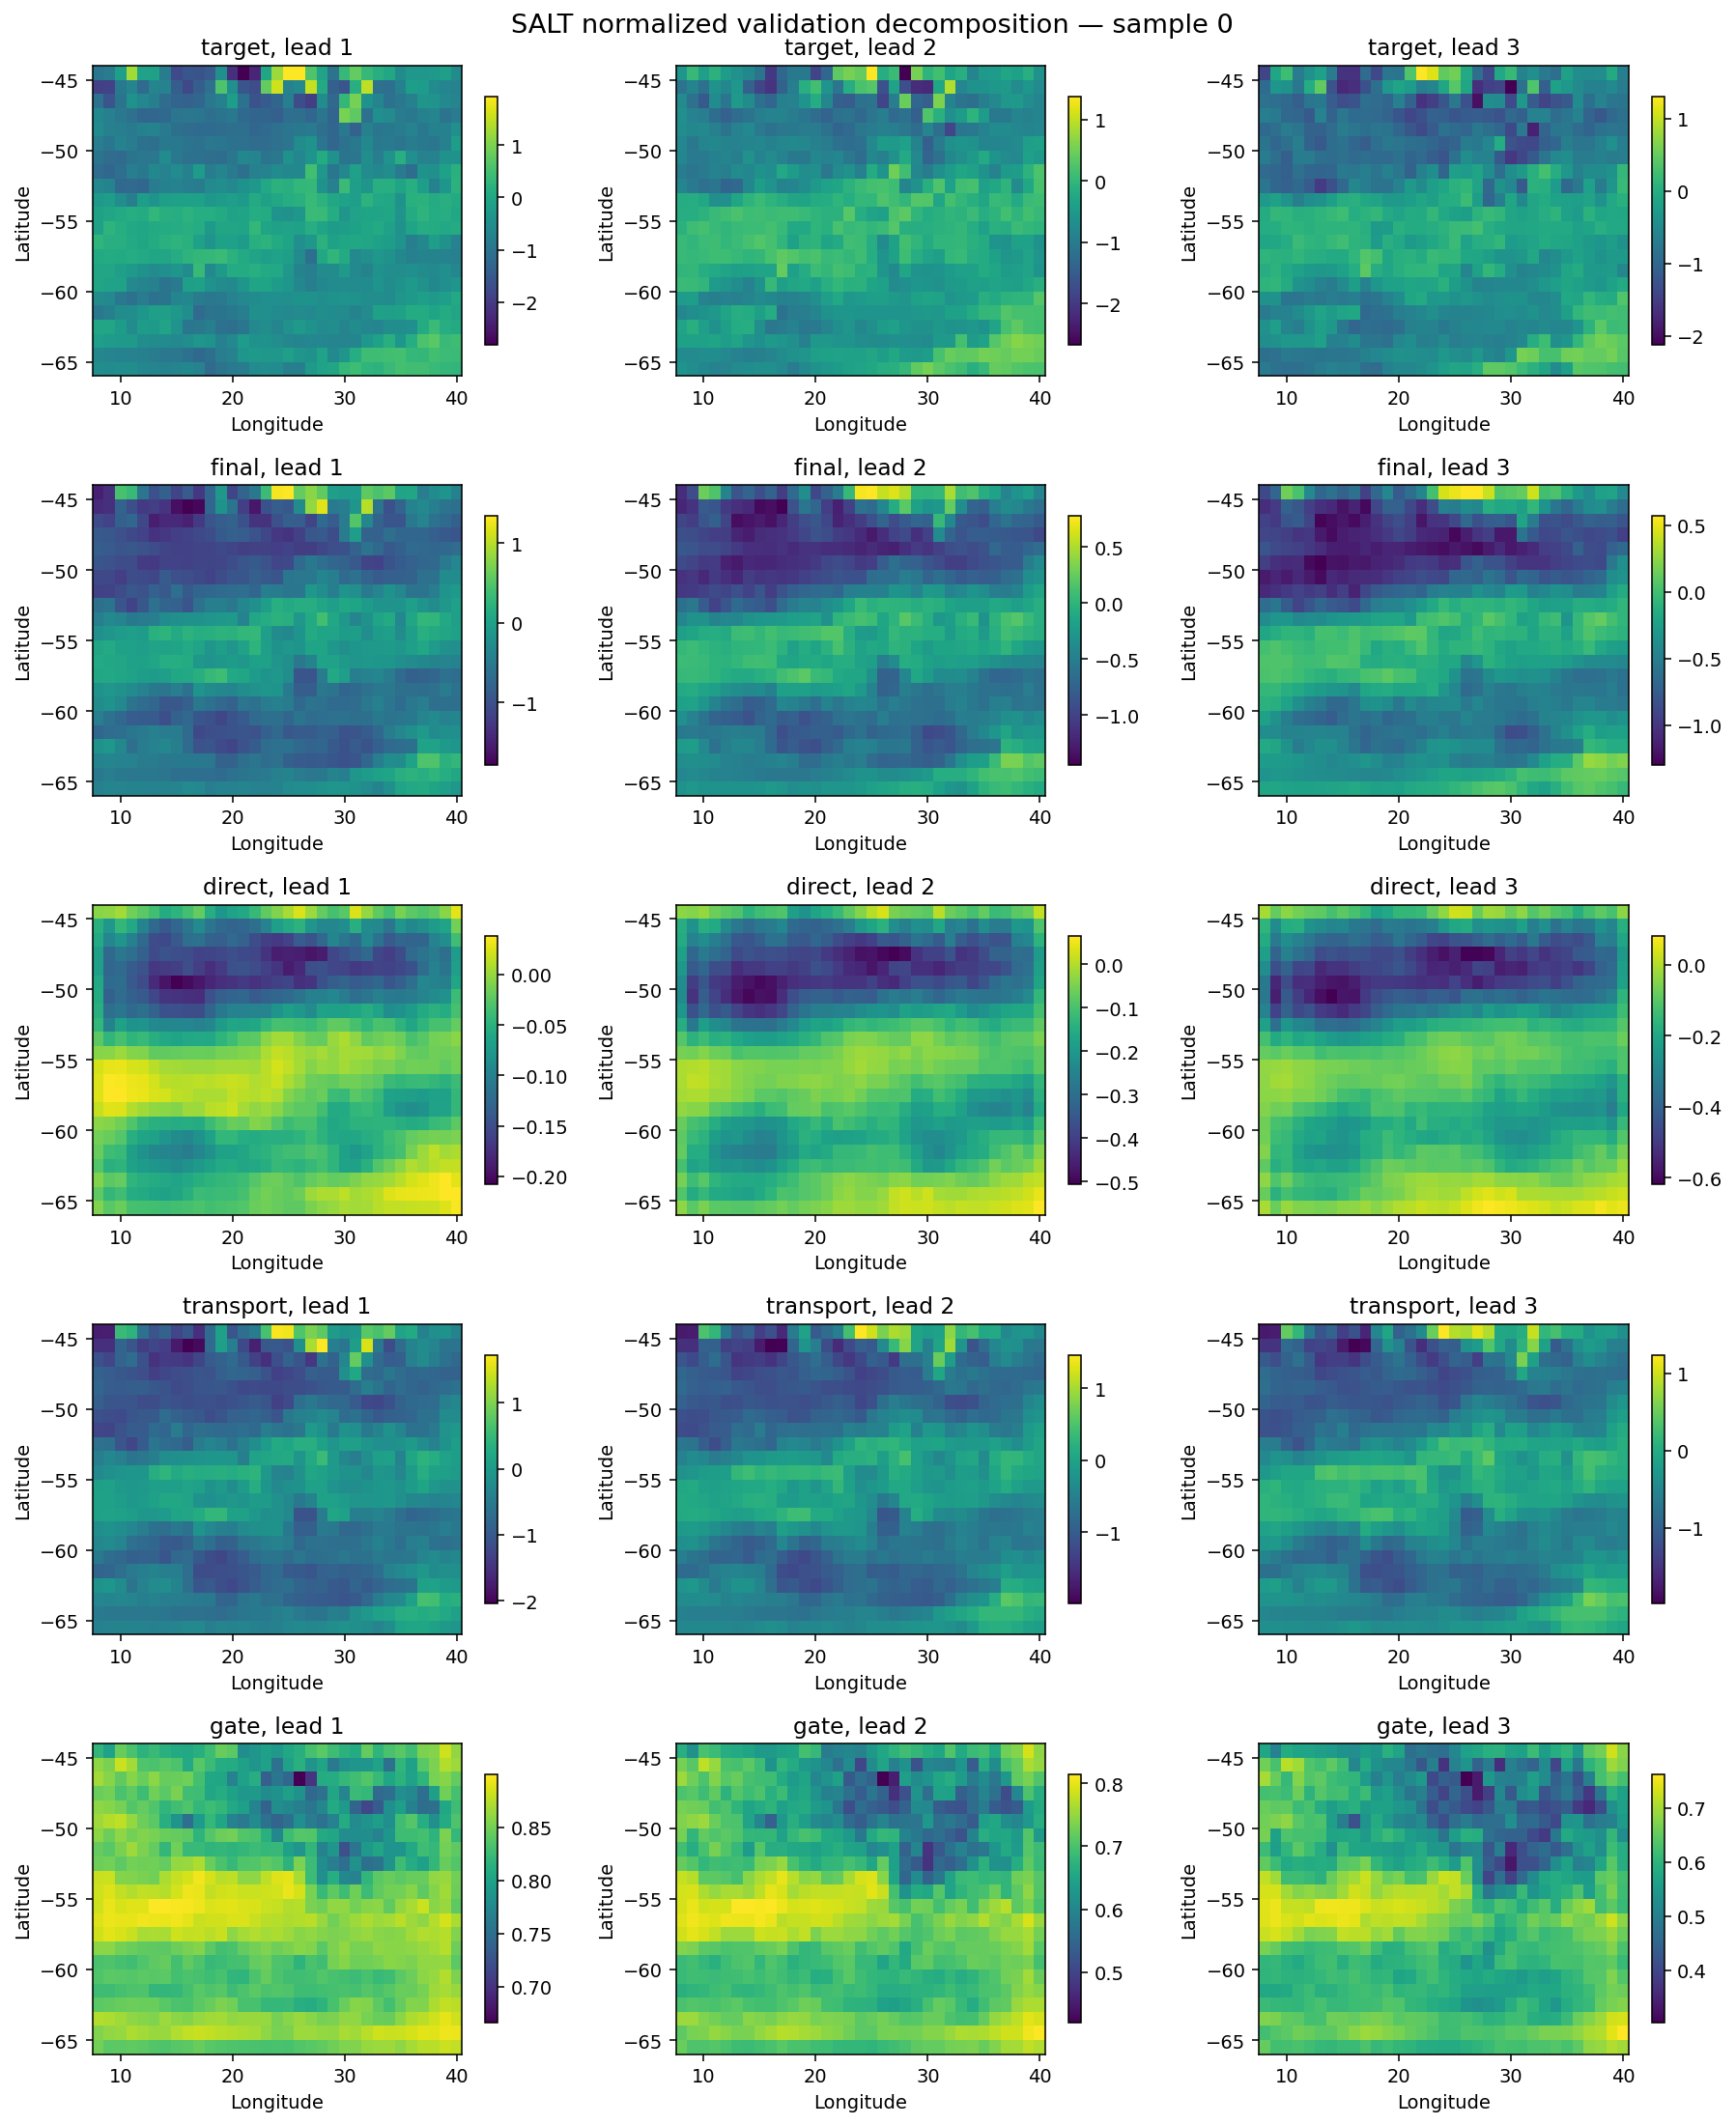
\includegraphics[width=0.46\textwidth]{dynaseaf_validation_salt_panel}}
\caption{Qualitative validation branch diagnostics for the full DynaSEAF model at seed 42 and one validation origin--window sample. Each panel shows the target, fused final forecast, direct branch, transported branch, and target-resolved gate for the first three forecast leads. These maps are validation diagnostics, not test samples and not inputs to checkpoint selection.}
\label{fig:dynaseaf_validation_decomposition}
\end{figure*}

\section{Discussion}

\subsection{Evidence Synthesis}
The frozen DynaSEAF model improves the validation aggregate over its SEAF-v1 backbone: Macro $\mathrm{SS}_{\mathrm{AP}}$ increases from $0.3176\pm0.0023$ to $0.3637\pm0.0018$, and Macro $\mathrm{SS}_{\mathrm{DAP}}$ increases from $0.1646\pm0.0033$ to $0.2170\pm0.0022$. On the held-out test split, DynaSEAF retains positive skill with Macro $\mathrm{SS}_{\mathrm{AP}}=0.3522\pm0.0052$ and Macro $\mathrm{SS}_{\mathrm{DAP}}=0.2040\pm0.0066$. The direct-anomaly target remains a first-order modeling decision, as shown by the backbone-controlled target contrasts. The focused validation screen identifies transport as the clearest sensitivity in the per-sample/per-lead diagnostic average, while the full-model aggregate remains the primary three-seed result.

DynaSEAF's dynamics-guided transport refinement provides the main structured hypothesis for how anomaly information evolves. The residual correction and adaptive gate support this refinement but are treated as implementation details rather than independent contributions. The validation diagnostics make the complete forward path inspectable through branch outputs, gates, deformation magnitudes, and predicted dynamics, but their single-seed screen should not be confused with a significance test or with the held-out test evaluation. We also do not interpret the inherited LCFF contrast as evidence for any individual DynaSEAF mechanism.

\subsection{Position Relative to Learned Baselines}
The learned-adapter comparison is numerically favorable to DynaSEAF on both reported splits: it has the highest mean TEMP/SALT skill and persistence-relative skill among the listed models. These models are not parameter matched: DynaSEAF has 5.09 million parameters, compared with 4.97 million for SEAF-v1 and 20.05--61.62 million for the learned adapters. The comparison supports a compact competitive architecture, but it does not establish universal superiority, statistical superiority over the learned adapters, or a causal role for parameter count.

\subsection{Limitations}
The evaluation has six main limitations. It uses one monthly reanalysis product, so ORAS5 biases and representativeness errors are inseparable from forecast error. The five-month horizon and fixed spatial windows do not test longer-range prediction, global spherical geometry, or consistency across adjacent windows. The objective imposes no conservation, equation-of-state, or dynamical-balance constraints. The component screen and qualitative branch diagnostics are validation-only, use one seed, and summarize per-sample/per-lead diagnostics rather than global test metrics. The held-out test aggregate is consequently kept separate from mechanism interpretation. Finally, the test evaluation is a pre-specified three-seed comparison; independent products and observations, parameter-matched baselines, and longer-horizon diagnostics are still needed to assess generalization and operational relevance.

\section{Conclusion}

We introduced DynaSEAF, which extends direct anomaly forecasting with model-generated future dynamics, a learned effective transport branch, and a lightweight residual correction; an adaptive direct/transport gate controls their combination. Under the frozen ORAS5 protocol, the 5.09-million-parameter model reaches validation TEMP/SALT RMSE of $0.4940\pm0.0005$/$0.0755\pm0.0002$ and Macro $\mathrm{SS}_{\mathrm{AP}}/\mathrm{SS}_{\mathrm{DAP}}$ of $0.3637\pm0.0018$/$0.2170\pm0.0022$. On the held-out test split, it reaches $0.4750\pm0.0022$/$0.0762\pm0.0004$ and $0.3522\pm0.0052$/$0.2040\pm0.0066$, respectively. These results establish the DynaSEAF full-model baseline and its positive persistence-relative skill under the stated protocol.

The inherited anomaly target remains supported by controlled SEAF-v1 and Local CNN contrasts. The validation archive makes the DynaSEAF transport refinement and its supporting correction diagnostics inspectable and shows the strongest screen-level sensitivity for transport, while the held-out test aggregate provides the main generalization evidence. Independent ocean products, longer horizons, parameter-matched baselines, and deeper-ocean regimes remain important next steps.

\appendices
\section{Validation Ablation and Mechanism Evidence}
\label{sec:appendix_validation_ablation}
The validation archive contains the A0--A4 ladder and the component controls \texttt{no\_dynamics\_aux}, \texttt{no\_transport}, \texttt{no\_innovation}, and \texttt{no\_gate} at seed 42. Table~\ref{tab:dynaseaf_ablations_full} reports the complete origin--window-sample/per-lead normalized RMSE screen; the focused transport comparison is shown in Table~\ref{tab:dynaseaf_ablations}, and the three-seed global validation and held-out test aggregates remain in the main tables.

\begin{table}[!t]
\centering
\caption{Complete validation ablation screen for DynaSEAF (seed 42). Entries are means over validation origin--window samples and leads of normalized RMSE; lower is better. The focused transport comparison is shown in the main text; the remaining controls are retained here for completeness.}
\label{tab:dynaseaf_ablations_full}
\scriptsize
\setlength{\tabcolsep}{3.0pt}
\renewcommand{\arraystretch}{1.05}
\begin{tabular}{lccc}
\toprule
Configuration & TEMP $\downarrow$ & SALT $\downarrow$ & Macro $\downarrow$\\
\midrule
A0: SEAF-v1 & 0.8127 & 0.7354 & 0.7741\\
A1: dynamics only & 0.8147 & 0.7396 & 0.7771\\
A2: + transport & 0.7961 & 0.7203 & 0.7582\\
A3: + residual correction & 0.7989 & 0.7225 & 0.7607\\
A4: full DynaSEAF & 0.7980 & 0.7201 & 0.7591\\
\texttt{no\_dynamics\_aux} & 0.8014 & 0.7232 & 0.7623\\
\texttt{no\_transport} & 0.8198 & 0.7400 & 0.7799\\
\texttt{no\_innovation} & 0.7936 & 0.7206 & 0.7571\\
\texttt{no\_gate} & 0.7989 & 0.7225 & 0.7607\\
\bottomrule
\end{tabular}
\end{table}

The omitted controls are reported without independent contribution claims: they are single-seed validation diagnostics used to document the full configuration screen, not test-level evidence. The residual correction is evaluated through the matched counterfactual in Fig.~\ref{fig:dynaseaf_mechanism_validation}, rather than by treating its tensor as a standalone forecast.

Each diagnostic record is aligned to the forecast origin, region, variable, and lead. The archive includes the final forecast, direct forecast, transported forecast, residual correction (stored as the model's innovation tensor), gate, deformation, predicted future dynamics, and target metadata. The qualitative panels and mechanism statistics in Figs.~\ref{fig:dynaseaf_mechanism_validation} and~\ref{fig:dynaseaf_validation_decomposition} are validation-only diagnostics and are not used for checkpoint selection.
\FloatBarrier

\section*{Acknowledgment}
The authors thank the maintainers of the open-source scientific software and the ECMWF/ICDC data services used in this study.

% Keep the reference list compact enough to avoid an orphaned final page.
\makeatletter
\patchcmd{\thebibliography}{\footnotesize}{\scriptsize}{}{}
\makeatother
\bibliographystyle{IEEEtran}
\bibliography{reference}

\end{document}
